\chapter{Konzeption}
\label{ch:concept}

In diesem Kapitel werden die Schritte und Entscheidungen erläutert, die zur Erhebung der Daten, zum Training des Classifiers und für die spätere Anwendung notwendig sind.
Dazu werden vorab einige Entscheidungen und Anforderung an die zu entwickelnden Module geknüpft.

\section{Zwischenschritte}
\label{sec:steps}

Der Prozess bis zur fertigen Inbetriebnahme schließt folgende drei Schritte ein, die in dieser Reihenfolge abgeschlossen werden müssen:

\begin{description}
    \item[Data Engineering] Die Daten müssen erhoben und mit dem Deep Learning Modell in Einklang gebracht werden.
    Aus rohen Videos und strukturierten Annotationen werden Samples in ein einheitliches \gls{ml}-Datenset überführt.
    \item[Training] Es muss ein einheitlicher Trainingsablauf definiert werden, um die Ergebnisse einzelner Experimente vergleichen zu können.
    Dabei werden Metriken zur Evaluation der Modelle und zur Analyse von Konflikten erhoben.
    \item[Verifikation] Mithilfe des trainierten Klassifizierers werden Samples manuell verifiziert.
    Die Ground-Truth-Labels jener Samples, deren Fehler während des Trainings auffällig hoch sind, werden manuell verifiziert um so die Datenqualität zu verbessern.
    \item[Inferenz] Das trainierte Modell muss in eine Temporal Action Detection integriert werden, sodass ungeschnittene Videos ganzer Spiele verarbeitet werden können.
    Schließlich muss der Classifier in eine Nutzerschnittstelle integriert und bereitgestellt werden.
    Die Integration soll technisch ermöglicht werden, ist allerdings nicht mehr Bestandteil dieser Arbeit.
\end{description}

\section{Datenquellen}
\label{sec:datenquellen}

Essenziell für das Data-Engineering ist, dass die Trainingsdaten die richtigen Informationen enthalten, die es dem Modell erst ermöglichen notwendige Zusammenhänge zu abstrahieren.
Die Daten müssen genug Informationen enthalten, um die Spielaktion lernbar zu machen.
Zudem sollten die Daten ein möglichst diverses Spektrum und einen geringen Bias (siehe~\cite{Gugger20}) aufweisen und keine Ausrichtung auf spezielle Eigenschaften haben.
Aus den genannten Gründen wird sich dagegen entschieden nur Aufnahmen einer taktischen Kamera oder eines bestimmten Stadions zu verwenden.
Damit das \gls{har}-Modell ausreichend gut adaptiert werden kann, wird stattdessen der Versuch unternommen ein Datenset zu generieren, das Spiele verschiedener Mannschaften, Nationalitäten und Geschlechter beinhaltet.
Zudem soll das Videomaterial verschiedenen (TV-)Quellen zugrunde liegen, sodass sich das Modell nicht auf bestimmte Eigenschaften des Kameraschnitts (wie Art der Kameraführung, Wiederholungen, Einblendungen, Bildqualität) einschießt.

Diese Rohdaten werden anschließend in ein \gls{ml}-Datenset konvertiert.
Neuronale Netze lernen mit Samples $(X, Y)$, wobei $x \in X$ ein vierdimensionaler Video-Tensor und $y \in Y$ das Output-Label ist.
Alle Samples $x$ entsprechen multidimensionalen Matrizen (Tensoren) der Größe $x \in R^{C \times T \times S_x \times S_y}$, die sich aus $T$ Farbbildern ($C=3$) eines Clips zusammensetzen.
Die Labels entsprechen einem One-Hot-enkodiertem Vektor $y \in \{0, \dots, 1\}^K$.

Da diese Tensoren unkomprimiert bereits in einer kleinen Menge einen erheblichen Teil des Dateispeichers belegen, werden \gls{har}-Datensets in der Regel in einer strukturierten Form als CSV- oder JSON-Datei veröffentlicht.
Diese Dateien speichern neben dem Label einen nur den Verweis zu der Videoquelle (als Link oder ID) und Start \ggf Start- und Endmarkierungen, in denen sich die Aktion im Video ereignet.
Die rohen Videodaten sind also nicht direkter Bestandteil des Datensets, sondern werden erst zur Laufzeit nachgeladen.

Um ein eigenes, ausreichend großes Datenset zu erstellen, werden in dieser Arbeit mehrere Datenquellen kombiniert und in ein ähnliches Dateiformat überführt.
Dabei wird die Erhebung von Videomaterial $X$ und die Erhebung von Aktionsannotationen $Y$ separat betrachtet.

\subsection{Aktionsannotationen}
\label{subsec:aktionsannotationen}

Da Videomaterial von Fußballspielen durch öffentliche oder kommerzielle Video-Plattformen im Internet vergleichsweise einfach zu finden ist, liegt der Fokus bei der Generierung des Datensets primär im Beziehen akkurater Annotationen.
Die Annotationen müssen eine genaue zeitliche Auflösung haben, die mindestens im Sekundenbereich liegt.
Das liegt zum einen daran, dass Aktionen bei einem schnellen Spiel oft dicht aufeinander folgen und zum anderen daran, dass sich die Spielaktionen selbst nur wenige Sekunden lang sind.
Zusätzlich sollen Sie mehr Klassen als die bisherigen Datensets (SoccerNet und SoccerDB) einschließen.

Als Provider für Annotations wird an dieser Stelle auf \gls{sbod}\footnote{Da die Sammlung kontinuierlich erweitert wird, bezieht sich die Bezeichnung \gls{sbod} im Folgenden auf den Stand vom 16.07.2020}~\cite{Statsbomb20} zurückgegriffen.
Dabei handelt es sich um eine frei nutzbare Sammlung professioneller Annotation eines kommerziellen Anbieters.
Die Sammlung umfasst mehr als 28 Millionen detaillierte Annotationen aus 33 Oberkategorien zu 799 Spielen.
Die Spiele wurden zwischen 2003 und 2020 ausgetragen und beziehen sich auf zehn internationale Ligen -- davon drei aus dem Frauenfußball.
Jede der Oberkategorien hat teils zahlreiche zusätzliche Attribute, wodurch sich weitere Unterkategorien ableiten lassen.

In \gls{sbod} ist die Dauer einer Aktion, die mit einem Schuss oder Pass zusammenhängt definiert durch die Dauer, die der Ball zwischen Abspiel und Annahme (\bzw dem Rollen ins Aus oder Tor) zurücklegt.
Andere Aktionen, wie Tore oder Auswechslungen, sind (wie auch in SoccerNet) als Zeitpunkte definiert.
Damit alle Klassen in gleicher Weise durch Intervall repräsentiert werden können, wird ein angepasstes Zeitfenster gewählt.
Dieses ergibt sich aus einer Mindestdauer pro Event, die um den besagten Zeitpunkt oder Mittelpunkt des Intervalls aufgespannt wird.
Ist das Original-Zeitfenster größer als die Mindestdauer, bleibt das Intervall unverändert.

\subsubsection*{Aktionskatalog}

Die Auswahl erlernbarer Aktionsklassen zur Action Recognition wird eingeschränkt durch die Verfügbarkeit des Providers.
Eine übersichtliche Auflistung aller erfassten Aktionen ist online\footnote{https://github.com/statsbomb/open-data/raw/master/doc/Open\%20Data\%20Events\%20v4.0.0.pdf (Stand: 08.10.2020)} zu finden.
Darüber hinaus unterliegt die Auswahl einiger selbstauferlegter Kriterien:

\begin{description}
    \item[Visuelle Erkennbarkeit] Eine Aktion muss allein auf Basis visueller Reize innerhalb weniger Frames erkennbar sein.
    Die Klassen \code{Starting XI} oder \code{Tactical Shift} werden dadurch ausgeschlossen.
    \item[Mindestanzahl an Beispielen] Aktionen müssen mit einer Mindestanzahl an Annotationen repräsentiert sein, damit sie in neuartigen Situationen sicher wiedererkannt werden können.
    Die untere Grenze wird bei 50 Beispielen festgesetzt und schließt somit Klassen wie \code{Own Goal Against} aus.
    \item[Maximalanzahl an Beispielen] Einige Aktionen wie \code{Pass} und \code{Carry} sind dermaßen überrepräsentiert, dass sich praktische jeder dieser Aktionen mit mindestens einer weiteren Aktion zeitlich überlagert.
    Zudem erschwert es die abschließende Temporal Action Detection wenn mehrere gleiche Aktionen direkt hintereinander stattfinden:
    Wird \zB ein direkter Pass gespielt, erfolgt die Ballannahme gleichzeitig mit der Ballabgabe und es gibt keinen zeitlichen Puffer zwischen beiden \code{Pass}-Aktionen.
    Die hier verwendete Methodik kann solche Abfolgen von direkt folgender gleicher Aktionen also gar nicht auseinander halten und müsste sie als eine lange Aktion behandeln.
    \item[Objektive Regeln] Die Aktionen müssen durch ein eindeutiges Regelwerk definiert sein.
    Klassen wie \code{Pressure}, \code{Error} oder \code{Miscontrol} werden als zu subjektiv eingestuft und werden daher ebenfalls ausgeschlossen.
\end{description}

Eine abschließende Liste aller insgesamt 32 abgeleiteten Aktionsklassen ist in \autoref{ch:aktionskatalog} zu finden.

\subsection{Videomaterial}
\label{subsec:videomaterial}

Als erste Video-Datenquelle wird das öffentliche Datenset SoccerNet verwendet.
Die Videos zu den Spielen sind pro Halbzeit zugeschnitten und können separat heruntergeladen werden.
Die Spiele decken fünf europäische Ligen, sowie Spiele der UEFA Championsleague ab, die zwischen 2014 und 2017 ausgetragen wurden.
Die Videoqualität ist durchweg gut und liegt bei einer Auflösung von mindestens 720p (siehe~\cite{SoccerNet20}).
SoccerNet besteht neben 6,637 Annotationen aus 1,000 Videos zu 500 Fußballspielen, wovon sich 41 mit den Annotationen aus \gls{sbod} überschneiden.
Diese Menge wird im Vergleich zu anderen Datensets allerdings noch als deutlich zu klein eingeordnet (vgl. \autoref{tab:dataset}).

Daher wird der Großteil der Videos über öffentliche Kanäle der Video-Plattform YouTube bezogen.
Diese Videos sind nicht pro Halbzeit zugeschnitten und potenziell fehlerbehaftet (\zB durch herausgeschnittene Spielminuten oder eine abweichende Abspielgeschwindigkeit), was ein zusätzliches Pre-Processing erfordert (siehe \autoref{ch:data}).

\section{Relevante HAR-Modelle und Hyperparameter}
\label{sec:decisions}

Neben der passenden Datengrundlage werden im nächsten Schritt geeignete \gls{har}-Modelle und die zu optimierenden Hyperparameter ausgewählt.
Anforderungen an ein passendes \gls{har}-Modell ist primär eine hohe Accuracy.
Zudem muss der Modell-Code, sowie vortrainierte Gewichte öffentlich-zugänglich sein und die Architektur sollte eine schnelle Inferenz ermöglichen, da das Modell zur Temporal Action Detection mehrmals für jede Aktion angewandt werden muss.
Der letzte Punkt schließt Modelle, die auf die Berechnung von Optischen Fluss angewiesen sind, kategorisch aus.
Die Performance betreffend liefern die Modelle SlowFast, X3D, ir-CSN, NL-I3D, Hidden-Two-Stream und R2+1D die besten Ergebnisse.
Aus der Gruppe der 3D-ConvNets wird auf NL-I3D verzichtet, da es unter den Ergebnissen von SlowFast bleibt, welches ebenfalls mit Non-Local-Blöcken kombiniert werden kann.
Zudem wird ein vollwertiges 3D-ConvNet wie I3D als zu groß erachtet, als dass die passende Hardware für das Training bereitgestellt werden kann.
Außerdem wird das Hidden Two Stream Modell ausgeschlossen, da es zum einen vergleichsweise schwache Ergebnisse liefert und zum anderen das einzige Modell in dieser Liste ist, welches nur eine in C++ geschriebene Implementierung mit dem Deep Learning Framework Caffe~\cite{Jia14} bereitstellt.
Alle weiteren Modelle sind in dem Python-Framework PyTorch~\cite{Paszke19} verfügbar und eine gesonderte Test- und Entwicklungsumgebung würde zu zusätzlichem Implementationsaufwand führen, der in diesem Fall als nicht gerechtfertigt angesehen wird.
Aus der Gruppe der Group-Convolution-Modelle wird ir-CSN gewählt, da es eine höhere Accuracy aufweist als X3D.

\subsection{Hyperparameter}
\label{subsec:hyperparameter}

Durch die Wahl der Architektur ergibt sich das Zielformat, das durch ein \gls{ml}-Datenset bereitgestellt wird und dem \gls{har}-Modell als Input dient.
Entscheidende Parameter für das Zielformat sind die Auflösung $S$, die Samplingrate $\tau$ und die Anzahl der Frames $T$.
Die Referenzmodelle R2+1D-34, ip-CSN-152 und SlowFast-50 nutzen unterschiedliche Kombinationen dieser Werte, die sich allerdings nur auf vortrainierter Modelle beziehen.
Technisch sind alle Modelle durch den Einsatz eines dynamischen \pool-Layers in der Lage auch mehr Frames zu verarbeiten.
\autoref{tab:coverage} zeigt die Parameter, sowie die ursprüngliche Länge eines Clips (Clip-Dauer $\Delta$) bei einer Framerate von 25 \gls{fps}.

Die Clip-Dauer bezeichnet im Folgenden die Originallänge in Sekunden, die ein Clip im ursprünglichen Video einnimmt.
Manche Aktionen (bzw\. Aktivitäten) bestehen aus mehreren Unteraktionen und dauern daher länger als andere Aktionen.
Enthalten die Trainingsdaten zu kurze Samples, kann das Modell \uU nicht genug Informationen erfassen, um solche Klassen zu erkennen.
Das einzelne Bild eines schießenden Spielers kann \zB zur Klasse Torschuss oder aber auch zur Klasse Flanke gehören.

\begin{figure}
    \centering
    \csvreader[no head,tabular=|l|r|r|r|r|,
    table head=\hline,late after line=\\\hline]{tbl/coverage.csv}
    {1=\model,2=\s,3=\t,4=\sr,5=\d}
    {\model & \s & \t & \sr & \d}
    \caption[Samplingstrategien]{Samplingstrategien}
    \label{tab:coverage}
\end{figure}

Während in SoccerNet alle Spielaktionen als Events behandelt werden und nur mit einem Zeitpunkt annotiert sind, haben die Samples in SoccerDB eine Kontextlänge von 3 bis 30 Sekunden.
In \gls{sbod} haben Spielaktionen (ausgenommen die Klasse \emph{TACTICAL\_SHIFT}) eine Kontextlänge von 0 bis 75 Sekunden.
Allerdings dauern 94,2 \% der Aktionen weniger lang als 3 Sekunden und 99,4 \% weniger als 6 Sekunden.

Im Zuge dieser Arbeit soll $\Delta$ zum einen groß genug gewählt werden, um alle Aktionsklassen lernbar zu machen, zum anderen aber dennoch möglichst klein, um eine zusätzliche Long-term Feature Aggregation (siehe \autoref{sec:long-term-aggregation-frameworks}) zu vermeiden und den Aufwand so zu begrenzen.
Daher werden 3 und 6 Sekunden als untere und oberen Grenzen für $\Delta$ festgesetzt.

\section{Überschneidungen von Aktionen}
\label{sec:multi-label}

Der oben genannte Aktionskatalog hat mit insgesamt 32 Aktionsklassen das Potenzial einige Aktionen zu beinhalten die sich mit anderen zeitlich überschneiden.
Dazu zählt einerseits der Fall, dass zwei Aktionen von zwei verschiedenen Spielern tatsächlich zeitgleich ausgeführt werden.
Andererseits können abhängig von der Problembeschreibung \zB hierarchische Klassen definiert werden, sodass sich eine Klasse \code{penaltyKick} immer mit der Klasse \emph{footShot} überlagert.

Um die Signifikanz dieses Problems zu verdeutlichen wurden für verschiedene $\Delta$ untersucht, wie oft sich eine Klasse mit einer anderen überschneidet.
Eine dedizierte Grafik ist in \autoref{ch:overlaps} zu finden.
Die häufigsten Kombinationen sind folgende:

\begin{enumerate}
    \item \code{saved} mit \code{footShot}
    \item \code{penaltyKick} mit \code{goal}
    \item \code{badBehavior} mit \code{card}
    \item \code{goal} mit \code{footShot}
    \item \code{collected} mit \code{cross}
\end{enumerate}

\begin{figure}
    \centering
    \begin{subfigure}{.3\textwidth}
        \centering
        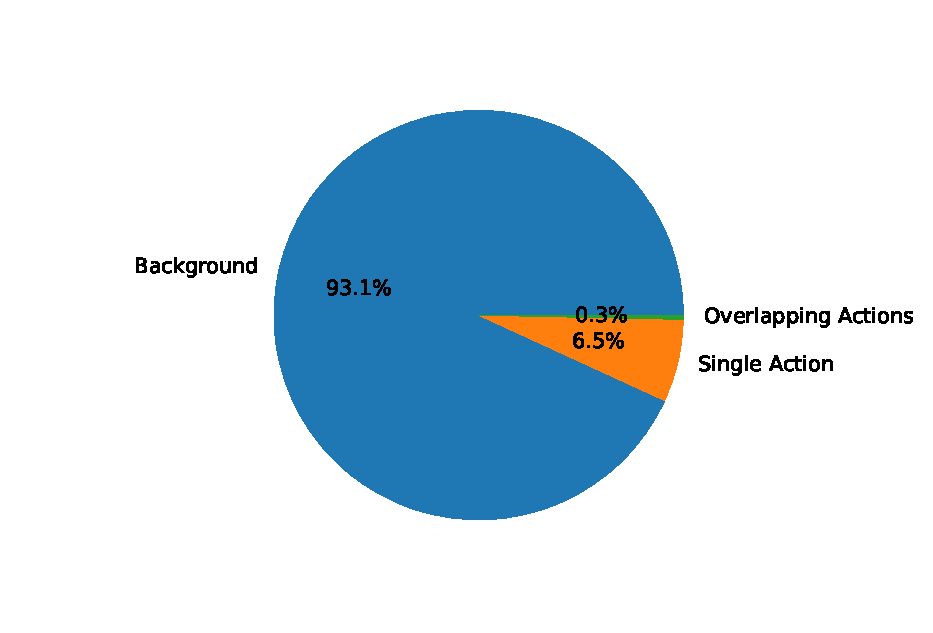
\includegraphics[width=.95\linewidth]{img/data-plots/1sec/background_ratio_all_1sek.eps}
        \caption{$\Delta = 1$}
        %\label{fig:anno_bg_ratio}
    \end{subfigure}%
    \begin{subfigure}{.3\textwidth}
        \centering
        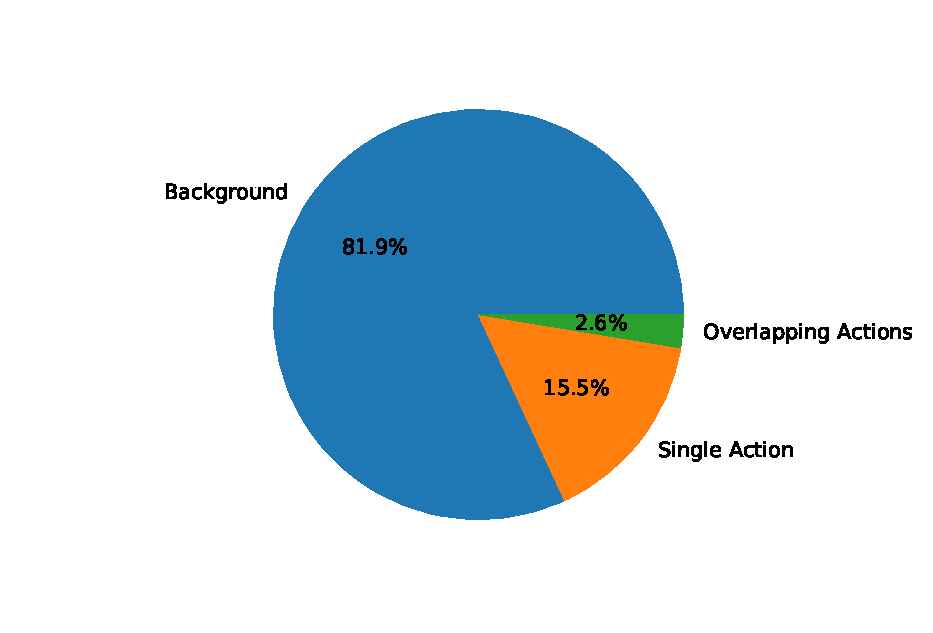
\includegraphics[width=.95\linewidth]{img/data-plots/4sec/background_ratio_all_202010-1419-3706.eps}
        \caption{$\Delta = 4$}
        %\label{fig:anno_classes}
    \end{subfigure}
    \begin{subfigure}{.3\textwidth}
        \centering
        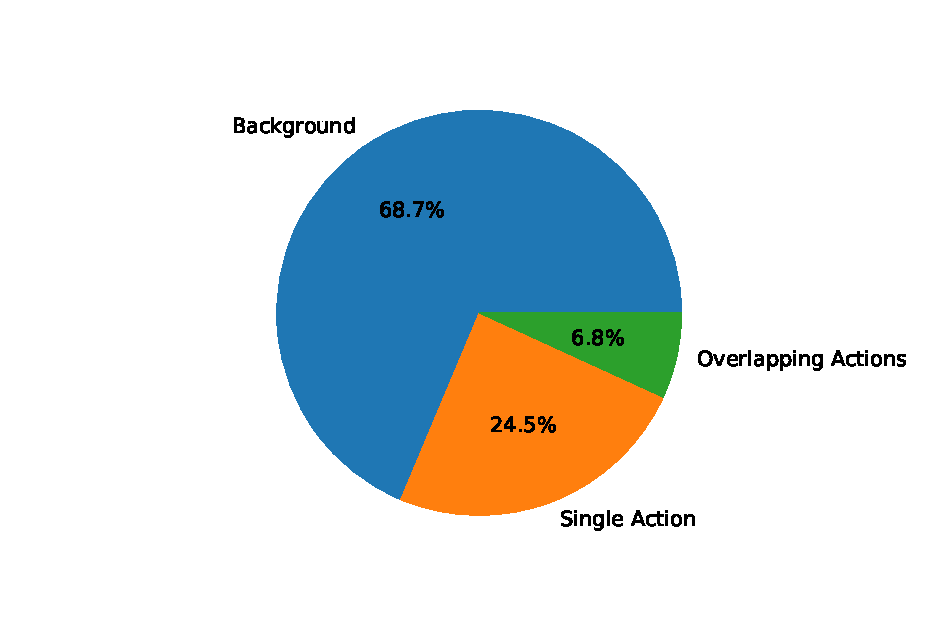
\includegraphics[width=.95\linewidth]{img/data-plots/8sec/background_ratio_all_202010-1419-4303.eps}
        \caption{$\Delta = 8$}
        %\label{fig:anno_classes}
    \end{subfigure}
    \caption{Skalierung des Background- und Überschneidungsverhältnisses zur Wahl von $\Delta$}
    \label{fig:ratios}
\end{figure}

Dass die Zahl der Überschneidungen mit der Wahl von $\Delta$ skaliert, belegt auch der wachsende Anteil von Samples mit mehr als einer Aktion, wie \autoref{fig:ratios} zeigt.
Dabei wird die in \autoref{subsec:segmentierung-und-sampling-strategie} verwendete Sampling-Strategie verwendet.

Als Folge der oben veranschaulichten Statistiken wird vorab auf ein Multi-Label-Ansatz gesetzt.
Das Verfahren ist damit auch flexibler bei Anpassungen des Aktionskatalogs und kommt ohne ein künstlichen \emph{Background}-Labels aus.
Zudem kann auf ein aufwendiges Verfahren dedizierte, überschneidungsfreie Intervalle für jede Aktion zu finden verzichtet werden.
Stattdessen kann das ungeschnittene Videomaterial gleichmäßig segmentiert werden und jedes Segment erhält Labels für alle darin stattfindenden Aktionen.

\section{Umgang mit Fehlern im Datenset}
\label{sec:umgang-mit-fehlern-in-datenset}

Auch wenn die Annotationen aus \gls{sbod} manuell erfasst und verifiziert wurden, können sie dennoch Fehler enthalten.
Und selbst bei gegebener Fehlerfreiheit läge ihnen wahrscheinlich ein anderes als das in dieser Arbeit verwendete Videomaterial zugrunde.
\gls{sbod} dient zur Auswertung von Spieldaten und ist auf Vollständigkeit aller Aktionen angewiesen.
Der grundlegende Unterschied zum Datenset dieser Arbeit ist, dass dieses Datenset ausschließlich sichtbare Aktionen umfassen soll.
Als Ground Truth gilt also immer nur das, was in dem jeweiligen Clip wirklich zu sehen ist.
\Dh zum einen, dass Aktionen die passiert sind, im Video aber nicht sichtbar sind (\zB weil die Kamera gerade ins Publikum schwenkt), entfernt werden müssen.
Zum anderen bedeutet es, dass Wiederholungen von Aktionen im Video zusätzliche Aktionen darstellen, auch wenn sie sich in der realen Welt zu einem anderen Zeitpunkt ereignet haben.

Aufgrund der zeitlichen Limitation dieser Arbeit kann nicht jeder Datensatz einzeln korrigiert werden.
Stattdessen wird ein Verifikationsschritt an bestimmten Zeitpunkten zwischen den Experimenten eingebaut.
Während des Trainings werden stets die Fehler der Loss-Funktion pro Sample protokolliert, sodass im Anschluss nur besonders auffällige Samples mit einem vergleichsweise hohen Fehlerwert manuell verifiziert und im Fehlerfall korrigiert werden müssen.
Der Ablauf orientiert sich an~\cite{Gugger20} und~\cite{Cioppa20}:
Letztere fanden durch die Ergebnisse der Loss-Funktion Fehler in den Annotationen von SoccerNet.

\section{Experimente}
\label{sec:experimente}

Im Zuge einiger Experimente soll geprüft werden, welche Architekturen besonders für die Klassifizierung von Spielaktionen geeignet sind, wie sich die Ergebnisse zusätzlich optimieren lassen und welche Klassen besonders schwer zu lernen sind.
Die Experimente lassen sich dabei in vier Phasen (siehe \autoref{fig:phases}) gliedern:

\begin{figure}[htbp!]
    \centering
    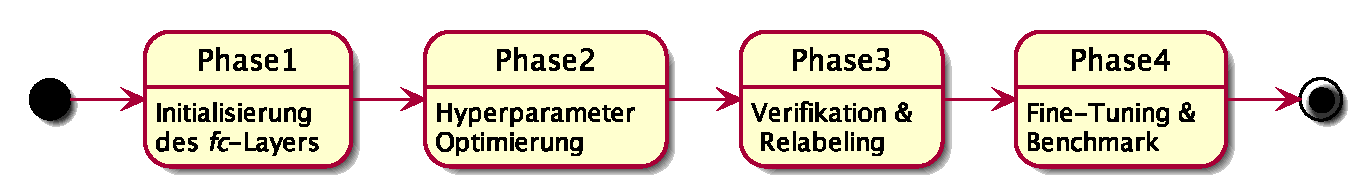
\includegraphics[width=0.9\textwidth, height=0.8\textwidth, keepaspectratio, interpolate]{fig/phases.eps}
    \caption{Ablauf der Experimente in vier Phasen}
    \label{fig:phases}
\end{figure}

Aufgrund von Hardwarebeschränkung können und sollen die Modelle nicht von Grund auf neu trainiert, sondern nur auf Basis vortrainierter Modelle nachtrainiert werden.
Kandidaten sind die bereits festgelegten Modelle SlowFast-50, ir-CSN-152 und R2+1D-34, die in der ersten Phase in Form eines einfachen Benchmarks verglichen werden.
Pro Modell findet zunächst in ein Initialisierungsschritt statt, in der die vortrainierten Gewichte (auf Basis von Kinetics) in die jeweilige Modellarchitektur geladen werden.
Da die vortrainierten Modelle mit anderen Klassen und mit deutlich mehr Klassen vortrainiert wurden, wird das hinterste \fc-Layer entfernt und durch ein neues \fc-Layer mit 32 Output-Knoten für die 32 Klassen von SOCC-HAR-32 ersetzt.
Die Gewichte des neuen \fc-Layers sind im Gegensatz zu den restlichen Layern zufällig initialisiert, was ein deutliches Ungleichgewicht der Wissensverteilung innerhalb des Netzes zur Folge hat~\cite{Gugger20}.
Um die Lücke zwischen Klassifikationslayer und dem Rest des Netzes zu verringern wird in diesem Schritt ausschließlich das \fc-Layer trainiert und alle anderen Layer werden während des Trainings eingefroren.
Nach Abschluss der Initialisierung ist das Wissen deutlich gleichmäßiger verteilt und jedes der Modelle kann auf allen Layern nachtrainiert werden.
Unter Berücksichtigung der Einschränkungen aus \autoref{sec:hardwareeinschrankungen} werden auch die restlichen Layer nachtrainiert.
Diese Ergebnisse dienen wiederum als Grundlage eines halbautomatisierten Verifikationsschritts.
Am Ende der ersten Phase wird schließlich die Entscheidung für eines der drei Baseline-Modelle gefällt, welches die besten Ergebnisse liefert und in den folgenden Phasen weiter optimiert wird.

In der zweiten Phase werden verschiedene Konfigurationen von Hyperparametern und damit verbundenen Werte für die Clip-Dauer getestet.
Da die Konfiguration der Pre-Trainings aus \autoref{tab:coverage} die untere Grenze von 3 Sekunden alle nicht erreichen, werden für jedes Modell die Hyperparameter $T$ und $\tau$ optimiert und somit auch ein längerer Kontext ermöglicht.
Technisch gesehen wird somit durch den Einsatz eines dünneren Samplings (mit steigendem $\tau$) \bzw dem Ausnutzen des dynamischen Avg-Pooling-Layers (mit steigendem $T$) eine Temporal Feature Aggregation umgesetzt.
Einige ausgewählte Kombinationen der Hyperarameter werden im Zuge einer Grid-Suche mit vergleichsweise wenig Trainingsdaten getestet.
Die beste Konfiguration wird schließlich mit zusätzlichen Daten weiter trainiert.

Der alternative Einsatz von \glspl{tsn} im Kontext dieser Arbeit wird als weniger geeignet eingeschätzt, da die Untersegmente eines Samples verschiedene Klassen beinhalten können.
Dieser Fall kann am Beispiel einer Wiederholung veranschaulicht werden:
Ein längerer Clip wird in drei Untersegmente geteilt, wovon eins eine Auswechslung und die anderen beiden eine Torwiederholung zeigen.
Im TSN würde der Clip als Tor klassifiziert werden, da diese Aktionen im Durchschnitt über alle drei Snippets öfter vertreten ist.
Da der Fehler über alle Snippets zurückpropagiert wird, würde das Netz während des Trainings so einen fehlerhaften Zusammenhang zwischen Tor und Auswechslung lernen.
\gls{tsn} ist also nur einsetzbar, wenn die Clips über seine komplette Länge nicht mit anderen Klassen interferiert.

In der dritten Phase werden die 32 Aktionsklassen einzeln evaluiert und Klassen, die nur extrem selten korrekt klassifiziert werden, werden aus dem ursprünglichen Datenset entfernt.
Da diese Klassen gravierenden Einfluss auf den Fehler und damit auf die Optimierung des Modells haben, wird das Netz erneut nachtrainiert mit nur einer Untermenge der ursprünglichen Klassen.
Auch hier folgt anschließend ein Verifikationsschritt.

In der letzten Phase werden weitere Verbesserungen der Metriken angestrebt, durch manuelle Anpassungen äußerer Parameter, Regularisierungstechniken (siehe \autoref{subsec:reaktive-aenderungen}), sowie durch spezielle Techniken, wie Label Smoothing~\cite{Szegedy16} oder Multi-Grid-Training~\cite{Wu20}.

Problematisch ist die Tatsache, dass die Modelle in den Experimenten verschieden lange Videos verarbeiten und sich die Trainings- und Validierungssets dadurch unterscheiden.
Zwar bleibt die Anzahl der Samples gleich, da immer ein Clip pro Sekunde gesamplet wird.
Die Labels pro Sample können jedoch bei verschiedener Länge abweichen.
Um trotzdem vergleichbare Ergebnisse zu erheben, wird zur Evaluation immer ein einheitliches Testset verwendet:
In der ersten Phase wird ein Testset mit $\Delta_\text{test}=3$ verwendet, da die maximale Clip-Dauer der drei Baseline-Modelle bei 2.67 Sekunden liegt.
In der zweiten Phase werden im Zuge der Hyperparameter-Optimierung auch längere Clips mit bis zu 6 Sekunden gesamplet, weshalb von dort an ein zweites Test-Set mit $\Delta_\text{test}=6$ verwendet wird.
Im Gegensatz zum Trainings- und Validierungsset unterliegen die Test-Sets keinem Downsampling.
\Dh die Ungleichgewichtungen der realen Welt (insbesondere die Überrepräsentation von Background-Samples) wird auch im Test-Set widergespiegelt.

%\subsubsection*{Vergleichbarkeit mit SoccerNet}

%Das einzige veröffentlichte Datenset im Bereich Fußball ist SoccerNet.
%Daher wird schließlich mit einem speziellen Test-Set evaluiert, das genau den Testdaten von SoccerNet entspricht.
%Die beste Architektur wird mit den vortrainierten Gewichten aus Phase XL übernommen und mit SoccerNet-500 nachtrainiert und mit dem Original Testset evaluiert.
%Dieses Set weist auch die gleichen negativen Einflussfaktoren auf, wie im Original:
%\item 3) Vergleichbarkeit: Überrepräsentation von Hintergrund von X, Fehlerhafte Annotationen, Nur eine Aktion pro Spielminute


\section{Modulare Implementation}
\label{sec:konzeptuelle-umsetzung}

Zur Umsetzung wurde auf ein modulares Framework gesetzt, das die Kernfunktionen für alle Zwischenschritte implementiert.

\begin{figure}[htbp!]
    \centering
    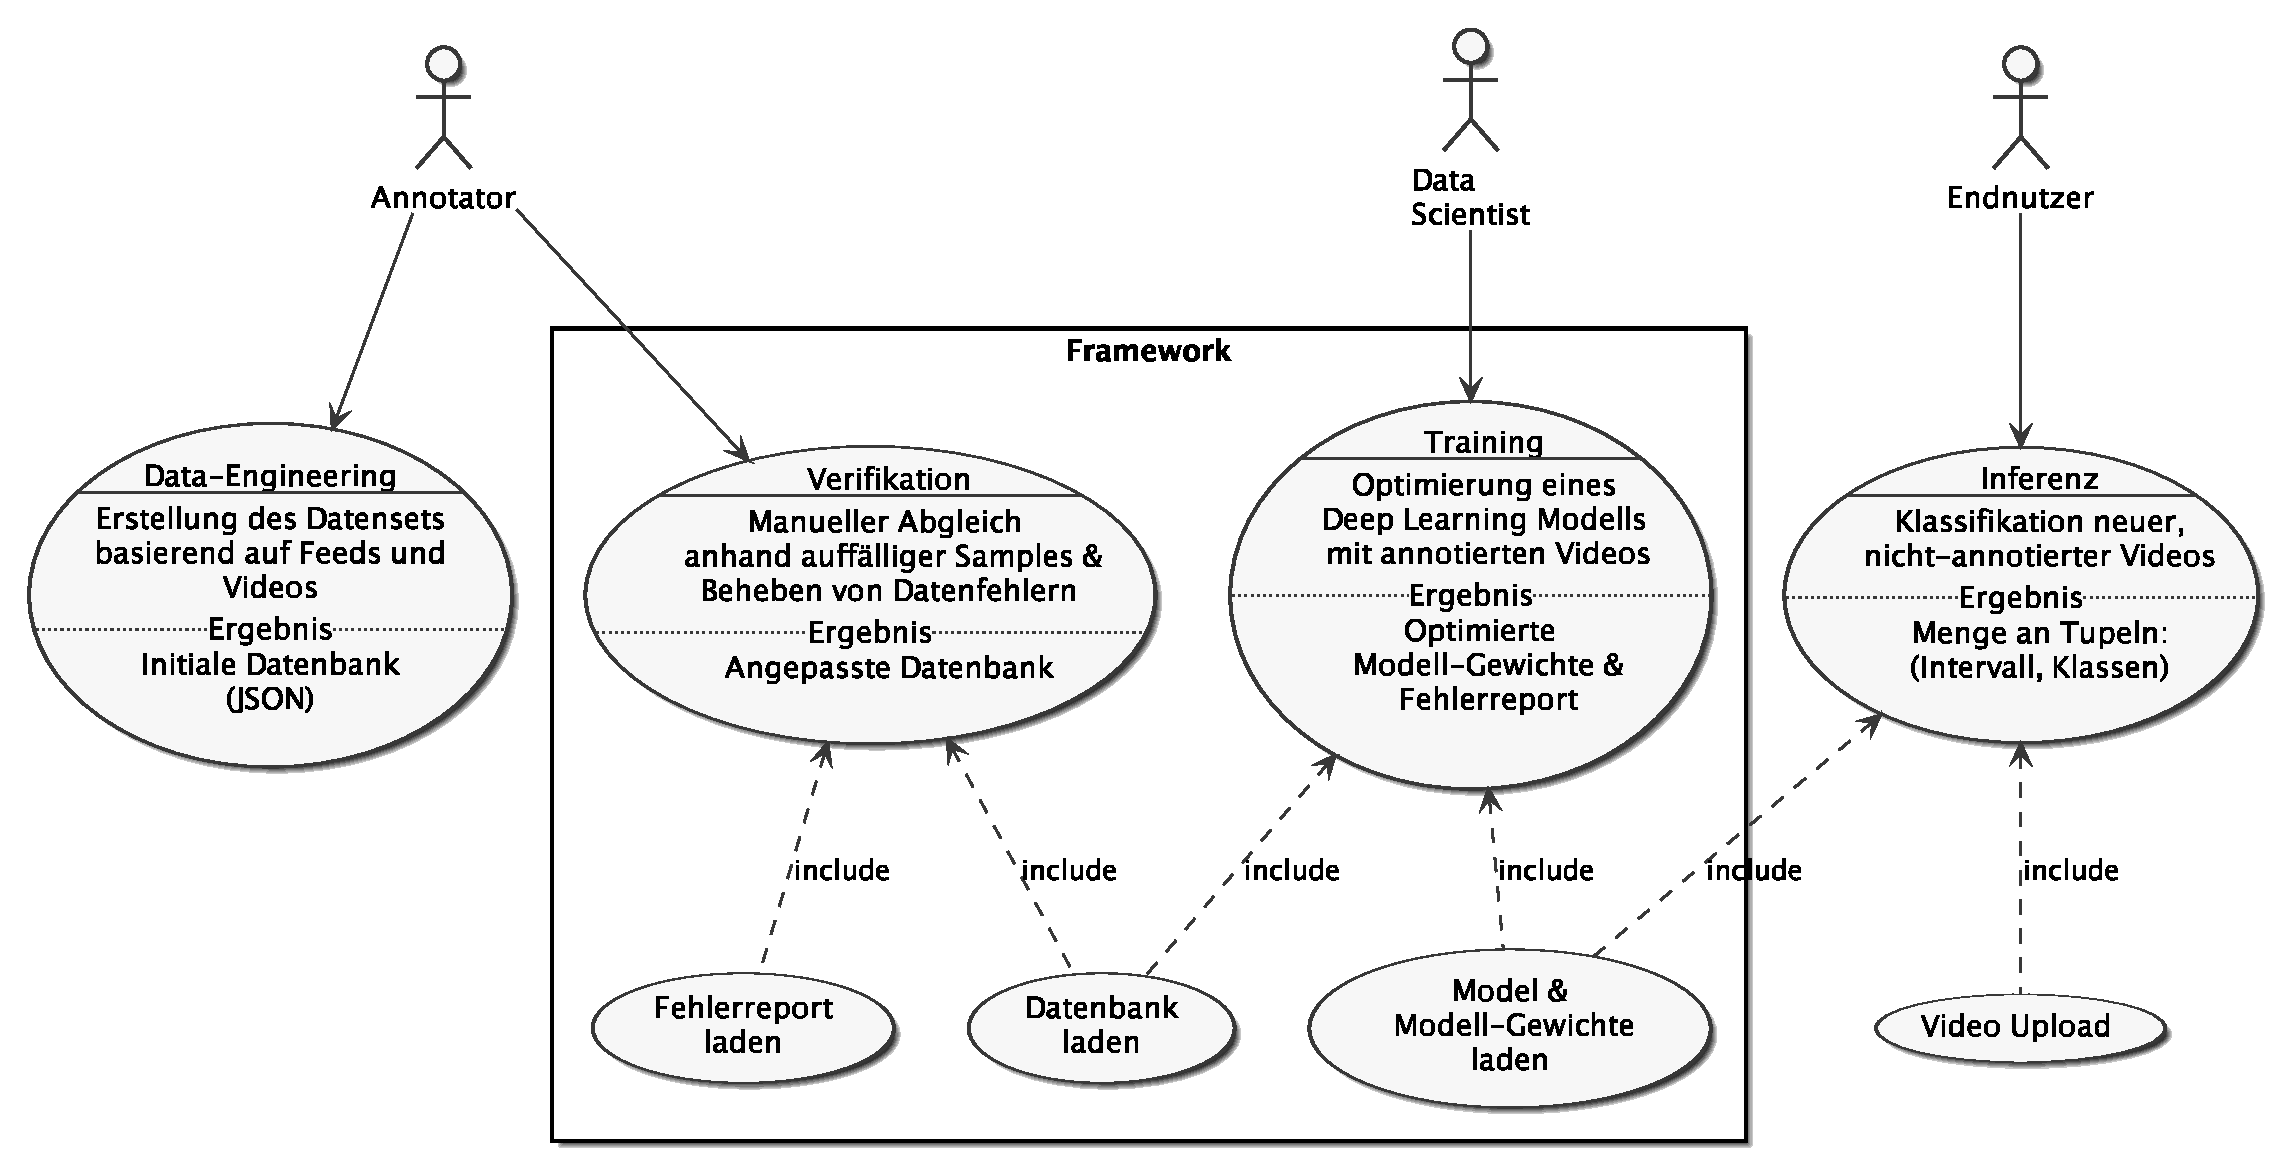
\includegraphics[width=0.9\textwidth, height=0.8\textwidth, keepaspectratio, interpolate]{fig/usecase.eps}
    \caption{Anwendungsfalldiagramm: Framework}
    \label{fig:usecase}
\end{figure}

\autoref{fig:usecase} zeigt die Anwendungsfälle aller Zwischenschritte, beginnend mit dem Data-Engineering, das vorab initial ausgeführt wird und die Trainingsdaten in einer Datenbank speichert.
Die Datenbank bildet die Import-Schnittstelle zu dem Framework, mit dem sich alle der vier, oben vorgestellten Phasen einheitlich zu durchlaufen lassen.
Während des Trainings die Trainingsdaten aus der Datenbank und die Modellgewichte aus entsprechenden Checkpoint-Dateien geladen.
Anhand der Trainingsdaten wird das Modell optimiert und die optimierten Gewichte werden als Ergebnis in neuen Checkpoint-Dateien persistiert.
Ebenso wird während des Trainings ein Fehlerreport erfasst, der pro Sample Informationen wie Scores und den jeweiligen Fehler der Loss-Funktion erfasst.
Dieser Report wird als weiteres Ergebnis persistiert.
Im Verifikationsschritt werden Checkpoints und Fehlerreport der potenziell besten Epoche geladen und auffällige Samples werden manuell verifiziert.
Das Ergebnis ist eine angepasste Version der initialen Datenbank, in der die erkannten Fehler behoben sind.
Der abschließende Schritt der Inferenz ist möglich mit der Export-Schnittstelle der Modellgewichte.
Das Framework schließt den vorgelagerten Zwischenschritt des Data-Engineering und den optionalen Schritt der Inferenz also nicht mit ein, stellt aber dennoch Schnittstellen für beide Prozesse zur Verfügung.


Um alle Experimente in einer generischen Umgebung durchzuführen wurde eine modulare Implementation umgesetzt, die auf den Konzepten des Frameworks Lightning (\cite{Falcon19}) basiert.
In \autoref{fig:modules} sind die drei Kernmodule zur Datenintegration, Training und Evaluierung schemenhaft veranschaulicht.

\begin{figure}
    \centering
    \bigimage{fig/modules-top}{0.8\textwidth}
    \caption{Module zur konzeptuellen Umsetzung}
    \label{fig:modules}
\end{figure}

Die Hyperparameter aus \autoref{subsec:hyperparameter} sind allesamt für das Datenmodul konfigurierbar.
Das Datenmodul beinhaltet Klassen zum Erstellen und Bereitstellen valider Samples, die auf Grundlage der Datenbank erzeugt und vom Training- und Evaluation-Modul in Form von Batches genutzt werden können.

Das Trainingsmodul nutzt diese Samples zur Optimierung des \gls{har}-Backbones.
Das Backbones-Modell ist dabei gegen jede andere Architektur austauschbar, sofern sie eine wohl-definierte Schnittstelle bereitstellt.
Während des Trainings werden Metriken, Checkpoint- und Fehlerreport-Dateien erfasst und an das Evaluationsmodul in Form eines Loggings übermittelt.

Das Evaluationsmodul sichert alle geloggten Daten zusammen mit weiteren Metadaten in einem Cloud-Speicher\footnote{Ergebnisse unter https://www.comet.ml/narendorf/soccar-32}.
Auch die Hyperparameter und der Quellcode werden pro Experiment in der Cloud gesichert, sodass sich alle Ergebnisse eindeutig reproduzieren lassen.
Zudem hat das Evaluationsmodule eine Funktion zur in \autoref{sec:umgang-mit-fehlern-in-datenset} beschriebenen Verifikation und kann basierend auf einem Fehlerreport die zugrunde liegende Datenbank anpassen.
